\question 设主存容量为1MB,外存容量为400MB,计算机系统的地址寄存器有24位,那么虚存的最大容量是(
)(默认字长为1B)
\par\twoch{1MB}{\textcolor{red}{16MB}}{17MB}{401MB}
\begin{solution}当外存容量足够大时,虚拟存储空间是只跟地址结构的位数相关的,即虚拟存储空间小于等于内存加上外存容量之和。
当外存容量不足时,外存容量也成为一个限制条件。即虚拟存储空间等于内存加上外存容量之和。
本题是外存容量足够大的情况,虚拟存储器的最大容量是由计算机的地址结构确定的,其虚拟地址空间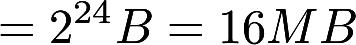
\includegraphics[width=1.28125in,height=0.16667in]{texmath/3bdb835Cdpi7B3507D3D25E7B247DB3D16MB}
\end{solution}
\question 在现代计算机系统中,存储器是十分重要的资源,能否合理有效地使用存储器在很大程度上反映了操作系统的性能,并直接影响到整个计算机系统作用的发挥。可以通过哪些途径来提高主存利用率(
)。 Ⅰ.将连续分配方式改为离散分配方式 Ⅱ.增加对换机制
Ⅲ.引入虚拟存储机制 Ⅳ.引入存储器共享机制
\par\twoch{Ⅰ、Ⅱ和Ⅲ}{Ⅰ、Ⅱ和Ⅳ}{Ⅱ、Ⅲ和Ⅳ}{\textcolor{red}{全是}}
\begin{solution}Ⅰ对,将连续分配方式改为离散分配方式以减少内存的零头。
Ⅱ对,增加对换机制,将那些暂时不能运行的进程或暂不需要的程序或数据换出至外存,以腾出内存来装入运行的程序。
Ⅲ对,引入虚拟存储机制,使更多的作业能够装入内存,提高CPU和内存利用率。
引入动态链接机制,当程序在运行中需要调用某段程序时才将该程序装入内存,从而避免装入不会用到的程序段和数据。
Ⅳ对,引入存储器共享机制,允许一个正文段或数据段被若干程序共享以消除内存中的重复拷贝现象。
\end{solution}
\question (浙江大学,2005年)外存加上内存之和与虚拟内存空间相比,其大小关系是
\par\twoch{前者比后者大}{前者比后者小}{二者相等}{\textcolor{red}{不一定}}
\begin{solution}当外存容量足够大时,虚拟存储空间只跟地址结构的位数相关,即虚拟存储空间小于等于内存加上外存容量之和。
当外存容量不足时,外存容量也成为一个限制条件。即虚拟存储空间等于内存加上外存容量之和。
因此二者大小关系是不确定的。
\end{solution}
\question 虚拟存储器的最大容量取决于
\par\twoch{内外存容量之和}{\textcolor{red}{计算机的地址结构}}{是任意的}{作业的地址空间}
\begin{solution}虚拟存储器的最大容量取决于计算机的地址结构,并不是任意的。例如,计算机是32位系统,则虚拟存储器的最大寻址空间就是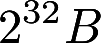
\includegraphics[width=0.36458in,height=0.15625in]{texmath/af718c5Cdpi7B3507D25E7B327DB},也就是虚拟存储器的最大容量。内外存的大小和作业的地址空间与虚拟存储器的大小没有直接关系,通常内外存的容量之和会小于或等于虚拟存储器的最大容量。
\end{solution}
\question (浙江大学,2006年)总体上说,``按需调页''(Demand-Paging)是个很好的虚拟内存管理策略。但是,有些程序设计技术并不适合于这种环境。例如
\par\twoch{堆栈}{线性搜索}{矢量运算}{\textcolor{red}{二分法搜索}}
\begin{solution}要使按需调页有效,就要紧紧抓住按需调页被提出的前提,那就是程序运行的局部性原理。按需调页适合运行的程序是具有局部性现象的程序,也就是最好是对数据进行顺序访问的程序。对于选项A,堆栈只能在栈顶进行操作,栈底的元素很久都用不着,显然对数据的访问具有局部性。对于选项B,线性搜索是按顺序搜索下来,显然也具有局部性。对于选项C,矢量运算就是数组运算,数组存放是连续的,所以数组运算就是邻近的数据的运算,也满足局部性。最后来看选项D,二分法搜索先查找中间的那个元素,如果没找到,再找前面数过去1/4位置或者倒数1/4位置的那个元素,再这样找下去,显然每次搜寻的元素不都是相邻的,二分法搜索是跳着搜索的,所以不具有局部性,不适合按需调页的环境,所以答案应该选D。
\end{solution}
\question 下面关于虚拟存储器的论述中,正确的是
\par\fourch{\textcolor{red}{在段页式系统中以段为单位管理用户的逻辑空间,以页为单位管理内存的物理空间,有了虚拟存储器才允许用户使用比内存更大的地址空间}}{为了提高请求分页系统中内存的利用率,允许用户使用不同大小的页面}{为了能让更多的作业同时运行,
通常只装入10\%~30\%的作业即启动运行}{最佳置换算法是实现虚拟存储器的常用算法}
\begin{solution}概念题,记住即可。在段页式系统中,段是用户的逻辑空间,页是内存的物理空间,因为段是用户定义的,而页是系统自动划分的,对于用户是透明的。每个系统的页面大小是固定的,由系统决定,不允许使用不同大小的页面。最佳置换算法仅用来对比其他算法,无法实现。
\end{solution}
\question 对36位虚拟地址的页式虚拟存储系统,每页8KB,每个页表项为32位,页表的总容量为
\par\twoch{1MB}{4MB}{8MB}{\textcolor{red}{32MB}}
\begin{solution}D。
根据虚拟地址的位数,可以得出虚存的容量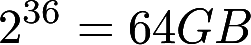
\includegraphics[width=0.89583in,height=0.16667in]{texmath/6eaeb55Cdpi7B3507D25E7B367D3D64GB},又根据页面大小为8KB,得出64GB/8KB=8M个页表项,每个页表项32位(4B),因此,页表的总容量为32MB。
归纳总结:主存空间和虚存空间都划分成若干个大小相等的页。主存即实存的页称为实页,虚存的页称为虚页。页表大小=页表项数
每个页表的字节数。
\end{solution}
